%%%%%%%%%%%%%%%%%%%%%%%%%%%%%%%%%%%%

\section{データの基礎}

%%%%%%%%%%%%%%%%%%%%%%%%%%%%%%%%%%%%

\subsection{観測値と変数}

\begin{frame}
\frametitle{クラスでのアンケート}

入門統計学の受講生を対象にアンケートが実施された。
以下はアンケートの質問の一部と、それに対応する変数名である：

\begin{itemize}
\item \var{gender}：あなたの性別は？
\item \var{intro\_extra}：自分を内向的・外向的、どちらだと思いますか？
\item \var{sleep}：平均して1日何時間寝ますか？
\item \var{bedtime}：ふだん何時頃就寝しますか？
\item \var{countries}：今までに何カ国訪れたことがありますか？
\item \var{dread}：この授業への「うんざり度」を1〜5で表すと？
\end{itemize}

\end{frame}

%%%%%%%%%%%%%%%%%%%%%%%%%%%%%%%%%%%%

\begin{frame}
\frametitle{データ行列}

統計学の受講生から様々な変数についてデータを収集した：

\begin{center}
\begin{tabular}{l cccc l}
		& \hl{変数} \\
		& \hl{$\downarrow$}	 \\
\cline{1-5}
学生	&	\var{gender}	&	\var{intro\_extra} & $\cdots$ & \var{dread} \\
\cline{1-5}
1 & male   & extravert  & $\cdots$  & 3 \\
2 & female & extravert  & $\cdots$  & 2 \\
3 & female & introvert  & $\cdots$  & 4 & \hl{$\leftarrow$}  \\
4 & female & extravert  & $\cdots$  & 2 & \hl{観測値} \\
$\vdots$	 &	$\vdots$	&	$\vdots$  &	$\vdots$ &	$\vdots$ \\
86	& male & extravert  & $\cdots$  & 3 \\
\cline{1-5}
\end{tabular}
\end{center}

\end{frame}

%%%%%%%%%%%%%%%%%%%%%%%%%%%%%%%%%%%%

\subsection{変数の種類}

\begin{frame}
\frametitle{変数の種類}

\begin{center}
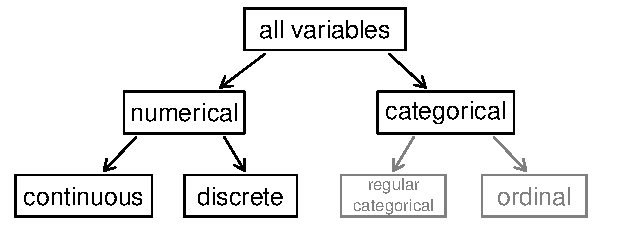
\includegraphics[width=0.9\textwidth]{1-2_data_basics/figures/variables/variables}
\end{center}

\end{frame}

%%%%%%%%%%%%%%%%%%%%%%%%%%%%%%%%%%%

\begin{frame}
\frametitle{変数の種類（続き）}

\begin{center}
{\footnotesize
\begin{tabular}{c ccc cc}
  \hline
 & \var{gender} & \var{sleep} & \var{bedtime} & \var{countries} & \var{dread} \\
  \hline
1 & male & 5 & 12-2 & 13 & 3 \\
  2 & female & 7 & 10-12 & 7 & 2 \\
  3 & female & 5.5 & 12-2 & 1 & 4 \\
  4 & female & 7 & 12-2 &  & 2 \\
  5 & female & 3 & 12-2 & 1 & 3 \\
  6 & female & 3 & 12-2 & 9 & 4 \\
  \hline
\end{tabular}
}
\end{center}

\begin{itemize}
\item \var{gender}：\soln{カテゴリ変数}
\item \var{sleep}：\soln{数値変数・連続}
\item \var{bedtime}：\soln{カテゴリ変数・順序}
\item \var{countries}：\soln{数値変数・離散}
\item \var{dread}：\soln{カテゴリ変数・順序尺度（数値変数として扱うことも可）}
\end{itemize}

\end{frame}

%%%%%%%%%%%%%%%%%%%%%%%%%%%%%%%%%%%

\begin{frame}
\frametitle{練習問題}

\pq{電話の市外局番はどのタイプの変数か？}

\begin{enumerate}[(a)]
\item 数値変数・連続
\item 数値変数・離散
\solnMult{カテゴリ変数}
\item カテゴリ変数・順序
\end{enumerate}

\end{frame}

%%%%%%%%%%%%%%%%%%%%%%%%%%%%%%%%%%%

\subsection{変数間の関係}

%%%%%%%%%%%%%%%%%%%%%%%%%%%%%%%%%%%

\begin{frame}
\frametitle{変数間の関係}

\dq{GPAと週の学習時間に関係はあるか？}

\begin{center}
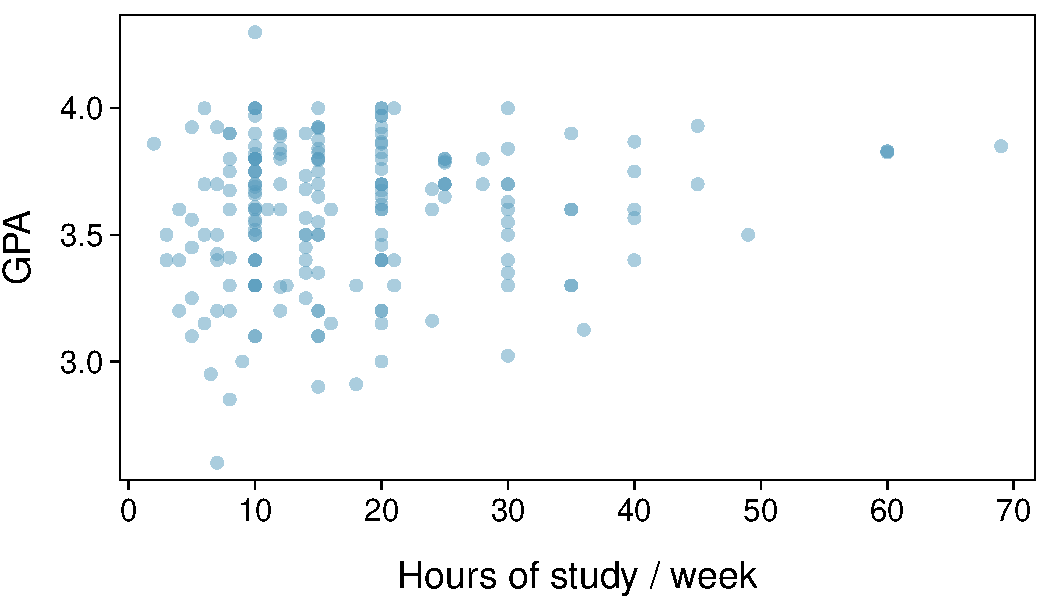
\includegraphics[width=0.7\textwidth]{1-2_data_basics/figures/gpa_study_hours/gpa_study_hours}
\end{center}

\dq{データ点に何か異常はないか？}

\soln{GPA$>$4.0の学生が1名おり、これはおそらくデータエラーである。}

\end{frame}

%%%%%%%%%%%%%%%%%%%%%%%%%%%%%%%%%%%

\subsection{説明変数と応答変数}

%%%%%%%%%%%%%%%%%%%%%%%%%%%%%%%%%%%

\begin{frame}
\frametitle{説明変数と応答変数}

\begin{itemize}

\item 2つの変数の組において説明変数を特定するには、
どちらがもう一方に影響を与えると考えられるかを判断する：

\begin{center}
説明変数 $\xrightarrow{\text{影響する可能性}}$ 応答変数
\end{center}

\item 変数を説明変数・応答変数と名付けても、
2変数間の関係が実際に因果関係であることを保証するわけではない。
関連が確認された場合でも同様である。
これらのラベルは、どちらがもう一方に影響を与えると予想されるかを
追跡するためだけに使う。

\end{itemize}

\end{frame}

%%%%%%%%%%%%%%%%%%%%%%%%%%%%%%%%%%%

\subsection{観察研究と実験の導入}

%%%%%%%%%%%%%%%%%%%%%%%%%%%%%%%%%%%

\begin{frame}
\frametitle{データ収集の2つの主要な方法}

\begin{itemize}

\item \hl{観察研究：}データが生じる過程に直接介入しない方法でデータを収集する（例：調査）。
\begin{itemize}
\item 変数間に自然に生じる関連の証拠を得ることはできるが、
それだけで因果関係を示すことはできない。
\end{itemize}

\item \hl{実験：}研究者が被験者をさまざまな処置にランダムに割り当て、
説明変数と応答変数の因果関係を確立する。

\end{itemize}

\end{frame}

%%%%%%%%%%%%%%%%%%%%%%%%%%%%%%%%%%%

\begin{frame}
\frametitle{相関と因果関係}

\begin{itemize}

\item 2つの変数が何らかの関係を示すとき、それらを\hl{関連した}変数と呼ぶ。
\begin{itemize}
\item 関連した変数は\hl{従属}変数とも呼ばれる。
\end{itemize}

\item 2つの変数が関連していない、すなわち明らかなつながりがない場合、
それらは\hl{独立}であると言う。

\item 一般に、\textbf{相関は因果関係を意味しない}。
因果関係はランダム化実験からのみ推論できる。

\end{itemize}

\begin{center}
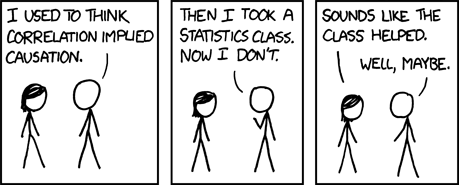
\includegraphics[width=0.55\textwidth]{1-2_data_basics/figures/xkcd_correlation} \\
{\tiny \webURL{http://xkcd.com/552/}}
\end{center}

\end{frame}

%%%%%%%%%%%%%%%%%%%%%%%%%%%%%%%%%%%%

\begin{frame}
\frametitle{練習問題}

\twocol{0.5}{0.5}
{
\pq{右の散布図に基づき、フクロモモンガの頭の長さと頭蓋骨の幅について正しい記述はどれか？}
}
{
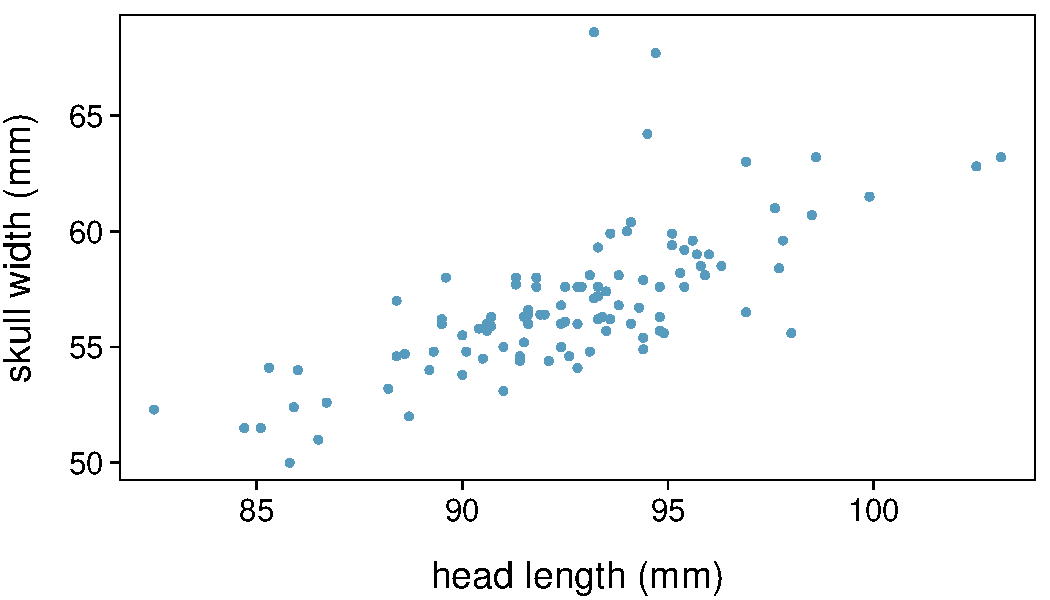
\includegraphics[width=\textwidth]{1-2_data_basics/figures/possum_head_skull/possum_head_skull}
}

\begin{enumerate}[(a)]
\item 頭の長さと頭蓋骨の幅に関係はなく、独立している。
\solnMult{頭の長さと頭蓋骨の幅は正の関連がある。}
\item 頭蓋骨の幅と頭の長さは負の関連がある。
\item 頭が長いほど頭蓋骨が広くなる（因果関係）。
\item 頭蓋骨が広いほど頭が長くなる（因果関係）。
\end{enumerate}

\end{frame}

%%%%%%%%%%%%%%%%%%%%%%%%%%%%%%%%%%%
